%structure taken from the fischsheet https://bitbucket.org/toman/fischsheet

%template by http://stdout.org/~winston/latex/

\documentclass[10pt,landscape,a4paper]{article}
\usepackage{multicol}
\usepackage{calc}
\usepackage{ifthen}
\usepackage[landscape]{geometry}
\usepackage{amsmath,amsthm,amsfonts,amssymb}
\usepackage{color,graphicx,overpic}
\usepackage{hyperref}
\usepackage{txfonts}
\usepackage[latin1]{inputenc}
\usepackage[T1]{fontenc}
\usepackage[ngerman]{babel}
\usepackage{listings}
\usepackage{pdfpages}
\lstset{tabsize = 3}


\pdfinfo{
  /Title (Cheatsheet #define true false)
  /Creator (TeX)
  /Author (Lukas, Quirin, Sebastian)
  /Subject (Cheatsheet for NWERC 2014)
}

% This sets page margins to .5 inch if using letter paper, and to 1cm
% if using A4 paper. (This probably isn't strictly necessary.)
% If using another size paper, use default 1cm margins.
\geometry{top=.45in,left=.5in,right=.5in,bottom=.5in}

% Turn off header and footer
\pagestyle{empty}

% Redefine section commands to use less space
\makeatletter
\renewcommand{\section}{\@startsection{section}{1}{0mm}%
                                {-1ex plus -.5ex minus -.2ex}%
                                {0.5ex plus .2ex}%x
                                {\normalfont\large\bfseries}}
\renewcommand{\subsection}{\@startsection{subsection}{2}{0mm}%
                                {-1explus -.5ex minus -.2ex}%
                                {0.5ex plus .2ex}%
                                {\normalfont\normalsize\bfseries}}
\renewcommand{\subsubsection}{\@startsection{subsubsection}{3}{0mm}%
                                {-1ex plus -.5ex minus -.2ex}%
                                {1ex plus .2ex}%
                                {\normalfont\small\bfseries}}
\makeatother

% Define BibTeX command
\def\BibTeX{{\rm B\kern-.05em{\sc i\kern-.025em b}\kern-.08em
    T\kern-.1667em\lower.7ex\hbox{E}\kern-.125emX}}

% Don't print section numbers
\setcounter{secnumdepth}{0}


\setlength{\parindent}{0pt}
\setlength{\parskip}{0pt plus 0.5ex}

%My Environments
\newtheorem{example}[section]{Example}
% -----------------------------------------------------------------------

\usepackage{fancyhdr}
\pagestyle{fancy}
\setlength{\headheight}{17pt} 
\lhead{Technische Universit\"at M\"unchen}
\rhead{\thepage}
\fancyfoot{}

\begin{document}
\raggedright
\footnotesize
\begin{multicols}{2}


% multicol parameters
% These lengths are set only within the two main columns
%\setlength{\columnseprule}{0.25pt}
\setlength{\premulticols}{1pt}
\setlength{\postmulticols}{1pt}
\setlength{\multicolsep}{1pt}
\setlength{\columnsep}{2pt}

\begin{center}
     \Large{
     	Team Reference Document\\
     	\underline{Team \#define true false, TU M\"unchen}\\
     	NWERC 2014} \\
\end{center}

\tableofcontents


\section{IO}
\subsection{C++ Input/Output/Limits}
\begin{lstlisting}[language=C++]
#include <iostream>
#include <iomanip>
#include <fstream>
#include <sstream>
#include <limits>
#include <algorithm>
#include <math.h>
#include <cstdlib>
#include <queue>
#include <vector>
#include <set>
#include <map>
#include <unordered_map>
#include <unordered_set>

using namespace std;
const int iMAX = numeric_limits<int>::max();
const int iMIN = numeric_limits<int>::min();
typedef long long LL;

int main() {
	// massively improve cout and cin performance for large streams
	ios::sync_with_stdio(false);
	cin.tie(0);
	
	// Ouput a specific number of digits past the decimal point, in this case 5    
	cout.setf(ios::fixed); cout << setprecision(5);
	cout << 100.0/7.0 << endl;
	cout.unsetf(ios::fixed);
    
	// Output the decimal point and trailing zeros
	cout.setf(ios::showpoint);
	cout << 100.0 << endl;
	cout.unsetf(ios::showpoint);
    
	// Output a '+' before positive values
	cout.setf(ios::showpos);
	cout << 100 << " " << -100 << endl;
	cout.unsetf(ios::showpos);
    
	// Output numerical values in hexadecimal
	cout << hex << 100 << " " << 1000 << " " << 10000 << dec << endl;
}
\end{lstlisting}
\section{Computations}
\subsection{Greates Common Divisor}

\begin{lstlisting}
long gcd(long a, long b)
{
if (b == 0)
return a;
else return gcd(b, a % b);
}
\end{lstlisting}

\subsection{Binomial Coefficients}

\begin{lstlisting}
long binomial(long n, long k)
{
if (k > n - k)
return binomial(n, n - k);

long result = 1;
if (k > n)
return 0;

for (long next = 1; next <= k; ++next)
{
long cancelled = gcd(result, next);
result = (result / cancelled)*(n - next + 1);
result = result/(next/cancelled);
}

return result;
}
\end{lstlisting}

\section{Data Structures}
\subsection{Union Find}
\begin{lstlisting}[language=C++]
initialize(): for all x, boss[x] = x, rank[x] = 0. 

union(x, y)
	a = find(x); b = find(y);
	if (rank(a) < rank(b)) boss[a] = b;
	if (rank(a) > rank(b)) boss[b] = a;
	if (rank(a) == rank(b)) {boss[b] = a; rank[a] += 1;}

find(x)
	if (boss[x] == x] return x;
	boss[x] = find(boss[x]); // path compression
	return boss[x];

\end{lstlisting}

\section{Math-Stuff}
\subsection{Euclid-Stuff}
\begin{lstlisting}[language=C++]
// This is a collection of useful code for solving problems that
// involve modular linear equations.  Note that all of the
// algorithms described here work on nonnegative integers.

typedef vector<int> VI;
typedef pair<int,int> PII;

// return a % b (positive value)
int mod(int a, int b) {
  return ((a%b)+b)%b;
}

// computes gcd(a,b)
int gcd(int a, int b) {
  int tmp;
  while(b){a%=b; tmp=a; a=b; b=tmp;}
  return a;
}

// computes lcm(a,b)
int lcm(int a, int b) {
  return a/gcd(a,b)*b;
}

// returns d = gcd(a,b); finds x,y such that d = ax + by
int extended_euclid(int a, int b, int &x, int &y) {  
  int xx = y = 0;
  int yy = x = 1;
  while (b) {
    int q = a/b;
    int t = b; b = a%b; a = t;
    t = xx; xx = x-q*xx; x = t;
    t = yy; yy = y-q*yy; y = t;
  }
  return a;
}

// finds all solutions to ax = b (mod n)
VI modular_linear_equation_solver(int a, int b, int n) {
  int x, y;
  VI solutions;
  int d = extended_euclid(a, n, x, y);
  if (!(b%d)) {
    x = mod (x*(b/d), n);
    for (int i = 0; i < d; i++)
      solutions.push_back(mod(x + i*(n/d), n));
  }
  return solutions;
}

// computes b such that ab = 1 (mod n), returns -1 on failure
int mod_inverse(int a, int n) {
  int x, y;
  int d = extended_euclid(a, n, x, y);
  if (d > 1) return -1;
  return mod(x,n);
}

// Chinese remainder theorem (special case): find z such that
// z % x = a, z % y = b.  Here, z is unique modulo M = lcm(x,y).
// Return (z,M).  On failure, M = -1.
PII chinese_remainder_theorem(int x, int a, int y, int b) {
  int s, t;
  int d = extended_euclid(x, y, s, t);
  if (a%d != b%d) return make_pair(0, -1);
  return make_pair(mod(s*b*x+t*a*y,x*y)/d, x*y/d);
}

// Chinese remainder theorem: find z such that
// z % x[i] = a[i] for all i.  Note that the solution is
// unique modulo M = lcm_i (x[i]).  Return (z,M).  On 
// failure, M = -1.  Note that we do not require the a[i]'s
// to be relatively prime.
PII chinese_remainder_theorem(const VI &x, const VI &a) {
  PII ret = make_pair(a[0], x[0]);
  for (int i = 1; i < x.size(); i++) {
    ret = chinese_remainder_theorem(ret.second, ret.first, x[i], a[i]);
    if (ret.second == -1) break;
  }
  return ret;
}

// computes x and y such that ax + by = c; on failure, x = y =-1
void linear_diophantine(int a, int b, int c, int &x, int &y) {
  int d = gcd(a,b);
  if (c%d) {
    x = y = -1;
  } else {
    x = c/d * mod_inverse(a/d, b/d);
    y = (c-a*x)/b;
  }
}

int main() {
  
  // expected: 2
  cout << gcd(14, 30) << endl;
  
  // expected: 2 -2 1
  int x, y;
  int d = extended_euclid(14, 30, x, y);
  cout << d << " " << x << " " << y << endl;
  
  // expected: 95 45
  VI sols = modular_linear_equation_solver(14, 30, 100);
  for (int i = 0; i < (int) sols.size(); i++) cout << sols[i] << " "; 
  cout << endl;
  
  // expected: 8
  cout << mod_inverse(8, 9) << endl;
  
  // expected: 23 56
  //           11 12
  int xs[] = {3, 5, 7, 4, 6};
  int as[] = {2, 3, 2, 3, 5};
  PII ret = chinese_remainder_theorem(VI (xs, xs+3), VI(as, as+3));
  cout << ret.first << " " << ret.second << endl;
  ret = chinese_remainder_theorem (VI(xs+3, xs+5), VI(as+3, as+5));
  cout << ret.first << " " << ret.second << endl;
  
  // expected: 5 -15
  linear_diophantine(7, 2, 5, x, y);
  cout << x << " " << y << endl;
}
\end{lstlisting}
\subsection{Gauss-Jordan}

\begin{lstlisting}
// Gauss-Jordan elimination with full pivoting.
//
// Uses:
//   (1) solving systems of linear equations (AX=B)
//   (2) inverting matrices (AX=I)
//   (3) computing determinants of square matrices
//
// Running time: O(n^3)
//
// INPUT:    a[][] = an nxn matrix
//           b[][] = an nxm matrix
//
// OUTPUT:   X      = an nxm matrix (stored in b[][])
//           A^{-1} = an nxn matrix (stored in a[][])
//           returns determinant of a[][]

#include <iostream>
#include <vector>
#include <cmath>

using namespace std;

const double EPS = 1e-10;

typedef vector<int> VI;
typedef double T;
typedef vector<T> VT;
typedef vector<VT> VVT;

T GaussJordan(VVT &a, VVT &b) {
  const int n = a.size();
  const int m = b[0].size();
  VI irow(n), icol(n), ipiv(n);
  T det = 1;

  for (int i = 0; i < n; i++) {
    int pj = -1, pk = -1;
    for (int j = 0; j < n; j++) if (!ipiv[j])
      for (int k = 0; k < n; k++) if (!ipiv[k])
	if (pj == -1 || fabs(a[j][k]) > fabs(a[pj][pk])) { pj = j; pk = k; }
    if (fabs(a[pj][pk]) < EPS) { cerr << "Matrix is singular." << endl; exit(0); }
    ipiv[pk]++;
    swap(a[pj], a[pk]);
    swap(b[pj], b[pk]);
    if (pj != pk) det *= -1;
    irow[i] = pj;
    icol[i] = pk;

    T c = 1.0 / a[pk][pk];
    det *= a[pk][pk];
    a[pk][pk] = 1.0;
    for (int p = 0; p < n; p++) a[pk][p] *= c;
    for (int p = 0; p < m; p++) b[pk][p] *= c;
    for (int p = 0; p < n; p++) if (p != pk) {
      c = a[p][pk];
      a[p][pk] = 0;
      for (int q = 0; q < n; q++) a[p][q] -= a[pk][q] * c;
      for (int q = 0; q < m; q++) b[p][q] -= b[pk][q] * c;      
    }
  }

  for (int p = n-1; p >= 0; p--) if (irow[p] != icol[p]) {
    for (int k = 0; k < n; k++) swap(a[k][irow[p]], a[k][icol[p]]);
  }

  return det;
}

int main() {
  const int n = 4;
  const int m = 2;
  double A[n][n] = { {1,2,3,4},{1,0,1,0},{5,3,2,4},{6,1,4,6} };
  double B[n][m] = { {1,2},{4,3},{5,6},{8,7} };
  VVT a(n), b(n);
  for (int i = 0; i < n; i++) {
    a[i] = VT(A[i], A[i] + n);
    b[i] = VT(B[i], B[i] + m);
  }
  
  double det = GaussJordan(a, b);
  
  // expected: 60  
  cout << "Determinant: " << det << endl;

  // expected: -0.233333 0.166667 0.133333 0.0666667
  //           0.166667 0.166667 0.333333 -0.333333
  //           0.233333 0.833333 -0.133333 -0.0666667
  //           0.05 -0.75 -0.1 0.2
  cout << "Inverse: " << endl;
  for (int i = 0; i < n; i++) {
    for (int j = 0; j < n; j++)
      cout << a[i][j] << ' ';
    cout << endl;
  }
  
  // expected: 1.63333 1.3
  //           -0.166667 0.5
  //           2.36667 1.7
  //           -1.85 -1.35
  cout << "Solution: " << endl;
  for (int i = 0; i < n; i++) {
    for (int j = 0; j < m; j++)
      cout << b[i][j] << ' ';
    cout << endl;
  }
}
\end{lstlisting}
\subsection{Collected Binomials}

\begin{lstlisting}
  //Berechnet alle Binomialkoeffizienten (n ueber k) mod m mit n<N
int binom[N][N];
void calcbinomials(int m) {
	for(int n=0; n<N; n++) {
		binom[n][0] = binom[n][n] = 1;
		for(int k=1; k<n; k++)
			binom[n][k] = (binom[n-1][k]+binom[n-1][k-1])%m;
	}
}
//Berechnet einzelnen Binomialkoeffizienten in Restklasse O(log n)
void calcbinom(int n, int k, int m) {
	return (fak[n] * inverse(fak[k], m) * inverse(fak[n-k], m))%m;
} //fak[n] = (n!)%m


//Berechnet fuer fixes n fuer alle k (n ueber k)  O(n)
void calcbinomrow(int n) {
	binom[n][0] = 1;
	for(int k=1; k<=n; k++) {
		binom[n][k] = binom[n][k-1]*(n-k+1)/k; //*inv(k) % MOD
	}
}
\end{lstlisting}


\section{Shortest Paths}
\subsection{Floyd-Warshall}
Floyd-Warshall kommt mit negativen Gewichten zurecht. All sources, all targets.
\begin{lstlisting}
procedure FloydWarshallWithPathReconstruction ()
    for k := 1 to n
       for i := 1 to n
          for j := 1 to n
              if (path[i][k] + path[k][j] < path[i][j]) {
                path[i][j] := path[i][k]+path[k][j];
                next[i][j] := next[i][k]; 
              }

 function Path (i,j)
    if path[i][j] equals infinity then
        return "no path";
    int intermediate := next[i][j];
    if intermediate equals 'null' then
        return " ";
    else
        return Path(i,intermediate) 
          + intermediate 
          + Path(intermediate,j);
\end{lstlisting}

\subsection{Dijkstra/Java}
\begin{lstlisting}[language=Java]
PriorityQueue<Item> q = new PriorityQueue<Item>();

Item[] index = new Item[n];
for(int i = 0; i < n; ++i) index[i] = new Item(-1, oo);

index[start] = new Item(-1, 0);
q.add(new Item(start, 0));

while(!q.isEmpty()) {
	Item curr = q.poll();
	if(curr.value > index[curr.node].value) continue;
	/*if(curr.node == end) break; */
	ArrayList<Item> edges = v.get(curr.node);
	for(int i = 0; i < edges.size(); ++i) {
		int nv = edges.get(i).value + curr.value;
		int otherNode = edges.get(i).node;
		Item oi = index[otherNode];
		if(nv < oi.value) {
			oi.value = nv;
			oi.node = curr.node;
			q.add(new Item(otherNode, nv));
		}
	}
}
return index;
\end{lstlisting}
\subsection{Bellman-Ford/Java}
\begin{lstlisting}
static class Item
{public int node;public double value;}

ArrayList<ArrayList<Item>> v = new ArrayList<ArrayList<Item>>(n);
for(int i = 0; i < n; ++i)
{
v.add(new ArrayList<Item>());
}
// Kanten einfuegen:
// v.get(a).add(new Item(b, c));
ArrayDeque<Integer> q = new ArrayDeque<Integer>();
Item[] index = new Item[n];
index[0] = new Item(-1, 0);
for(int i = 1; i < n; ++i)
{
index[i] = new Item(-1, oo);
}

boolean[] inQueue = new boolean[n];
inQueue[0] = true;
int phase = 0;
int nextPhaseStart = -1;
q.add(0);
boolean jackpot = false; // neg cycle
while(!q.isEmpty())
{
int i = q.poll();
inQueue[i] = false;
if(i == nextPhaseStart)
{
phase++;
nextPhaseStart = -1;
}
if(phase == n-1)
{
System.out.format("Case \#%d: Jackpot\n", numCase+1);
jackpot = true;
break;
}
Item it = index[i];
ArrayList<Item> e = v.get(i);
for(int x = 0; x < e.size(); ++x)
{
Item edge = e.get(x);
double nv = edge.value + it.value;
Item other = index[edge.node];
if(nv < other.value)
{
other.value = nv;
if(!inQueue[edge.node])
{
q.add(edge.node);
if(nextPhaseStart == -1)
{
nextPhaseStart = edge.node;
}
inQueue[edge.node] = true;
}
}
}
}
\end{lstlisting}

\vfill
\columnbreak
\section{Flow}
\subsection{MaxFlow Push-Relabel}

\begin{lstlisting}
#include <cmath>
#include <vector>
#include <iostream>
#include <queue>
using namespace std;
typedef long long LL;

struct Edge {
  int from, to, cap, flow, index;
  Edge(int from, int to, int cap, int flow, int index) :
    from(from), to(to), cap(cap), flow(flow), index(index) {}
};

struct PushRelabel {
  int N;
  vector<vector<Edge> > G;
  vector<LL> excess;
  vector<int> dist, active, count;
  queue<int> Q;

  PushRelabel(int N) : N(N), G(N), excess(N), dist(N), active(N), count(2*N) {}

  void AddEdge(int from, int to, int cap) {
    G[from].push_back(Edge(from, to, cap, 0, G[to].size()));
    if (from == to) G[from].back().index++;
    G[to].push_back(Edge(to, from, 0, 0, G[from].size() - 1));
  }

  void Enqueue(int v) { 
    if (!active[v] && excess[v] > 0) { active[v] = true; Q.push(v); } 
  }

  void Push(Edge &e) {
    int amt = int(min(excess[e.from], LL(e.cap - e.flow)));
    if (dist[e.from] <= dist[e.to] || amt == 0) return;
    e.flow += amt;
    G[e.to][e.index].flow -= amt;
    excess[e.to] += amt;    
    excess[e.from] -= amt;
    Enqueue(e.to);
  }
  
  void Gap(int k) {
    for (int v = 0; v < N; v++) {
      if (dist[v] < k) continue;
      count[dist[v]]--;
      dist[v] = max(dist[v], N+1);
      count[dist[v]]++;
      Enqueue(v);
    }
  }

  void Relabel(int v) {
    count[dist[v]]--;
    dist[v] = 2*N;
    for (int i = 0; i < G[v].size(); i++) 
      if (G[v][i].cap - G[v][i].flow > 0)
	dist[v] = min(dist[v], dist[G[v][i].to] + 1);
    count[dist[v]]++;
    Enqueue(v);
  }

  void Discharge(int v) {
    for (int i = 0; excess[v] > 0 && i < G[v].size(); i++) Push(G[v][i]);
    if (excess[v] > 0) {
      if (count[dist[v]] == 1) 
	Gap(dist[v]); 
      else
	Relabel(v);
    }
  }

  LL GetMaxFlow(int s, int t) {
    count[0] = N-1;
    count[N] = 1;
    dist[s] = N;
    active[s] = active[t] = true;
    for (int i = 0; i < G[s].size(); i++) {
      excess[s] += G[s][i].cap;
      Push(G[s][i]);
    }
    
    while (!Q.empty()) {
      int v = Q.front();
      Q.pop();
      active[v] = false;
      Discharge(v);
    }
    
    LL totflow = 0;
    for (int i = 0; i < G[s].size(); i++) totflow += G[s][i].flow;
    return totflow;
  }
};

\end{lstlisting}

\section{Matching}
\subsection{Max Bipartite Matching}

\begin{lstlisting}
#include <vector>

using namespace std;

typedef vector<int> VI;
typedef vector<VI> VVI;

bool FindMatch(int i, const VVI &w, VI &mr, VI &mc, VI &seen) {
  for (int j = 0; j < w[i].size(); j++) {
    if (w[i][j] && !seen[j]) {
      seen[j] = true;
      if (mc[j] < 0 || FindMatch(mc[j], w, mr, mc, seen)) {
        mr[i] = j;
        mc[j] = i;
        return true;
      }
    }
  }
  return false;
}

int BipartiteMatching(const VVI &w, VI &mr, VI &mc) {
  mr = VI(w.size(), -1);
  mc = VI(w[0].size(), -1);
  
  int ct = 0;
  for (int i = 0; i < w.size(); i++) {
    VI seen(w[0].size());
    if (FindMatch(i, w, mr, mc, seen)) ct++;
  }
  return ct;
}
\end{lstlisting}

\section{Graph Stuff}
\subsection{Strongly Connected Components}
\begin{lstlisting}
#include<vector>
 
using namespace std;
 
// Der Graph.
vector<int> g[20000];
// Anzahl der Knoten im Graphen.
int V;
 
// Interne Variablen fuer den Algorithmus
int d[20000], low[20000];
int t;
vector<int> stack;
bool instack[20000];
 
// Ergebnis-Struktur: enthaelt am Ende die starken 
//Zusammenhangskomponenten (als Listen von Knotenindizes)
vector<vector<int> > sccs;
 
void VISIT(int v) {
  d[v] = low[v] = ++t;
  stack.push_back(v);
  instack[v] = true;
  for (vector<int>::iterator w = g[v].begin(); w != g[v].end(); ++w) {
    if (! d[*w]) {
      VISIT(*w);
      low[v] = min(low[v], low[*w]);
    } else if (instack[*w]) {
      low[v] = min(low[v], low[*w]);
    }
  }
 
  if (d[v] == low[v]) {
    vector<int> scc;
    while(1) {
      int w = stack.back();
      stack.pop_back();
      instack[w] = false;
      scc.push_back(w);
      if (v == w)
        break;
    }
    sccs.push_back(scc);
  }
}
 
// Aufruf der VISIT Funktion:
memset(d, 0, sizeof(d));
memset(instack, 0, sizeof(instack));
t = 0;
for (int v = 0; v < V; v++)
  if (! d[v])
    VISIT(v);
\end{lstlisting}
\subsection{Topological Sort}
\begin{lstlisting}[language=C++]
void dsf(int x) {
	if(visited[x] {
		if(!f[x]) circle = true;
		return;
	}
	visited[x] = true;	

	for(Integer curr : list.get(x)) dsf(curr);

	out[tt] = x;
	tt++;
	f[x] = true;
}
\end{lstlisting}

\section{Strings}
\subsection{Suffix Array}
\begin{lstlisting}

#include <vector>
#include <iostream>
#include <string>

using namespace std;

struct SuffixArray {
  const int L;
  string s;
  vector<vector<int> > P;
  vector<pair<pair<int,int>,int> > M;

  SuffixArray(const string &s) : L(s.length()), s(s), P(1, vector<int>(L, 0)), M(L) {
    for (int i = 0; i < L; i++) P[0][i] = int(s[i]);
    for (int skip = 1, level = 1; skip < L; skip *= 2, level++) {
      P.push_back(vector<int>(L, 0));
      for (int i = 0; i < L; i++) 
	M[i] = make_pair(make_pair(P[level-1][i], i + skip < L ? P[level-1][i + skip] : -1000), i);
      sort(M.begin(), M.end());
      for (int i = 0; i < L; i++) 
	P[level][M[i].second] = (i > 0 && M[i].first == M[i-1].first) ? P[level][M[i-1].second] : i;
    }    
  }

  vector<int> GetSuffixArray() { return P.back(); }

  // returns the length of the longest common prefix of s[i...L-1] and s[j...L-1]
  int LongestCommonPrefix(int i, int j) {
    int len = 0;
    if (i == j) return L - i;
    for (int k = P.size() - 1; k >= 0 && i < L && j < L; k--) {
      if (P[k][i] == P[k][j]) {
	i += 1 << k;
	j += 1 << k;
	len += 1 << k;
      }
    }
    return len;
  }
};

int main() {

  // bobocel is the 0'th suffix
  //  obocel is the 5'th suffix
  //   bocel is the 1'st suffix
  //    ocel is the 6'th suffix
  //     cel is the 2'nd suffix
  //      el is the 3'rd suffix
  //       l is the 4'th suffix
  SuffixArray suffix("bobocel");
  vector<int> v = suffix.GetSuffixArray();
  
  // Expected output: 0 5 1 6 2 3 4
  //                  2
  for (int i = 0; i < v.size(); i++) cout << v[i] << " ";
  cout << endl;
  cout << suffix.LongestCommonPrefix(0, 2) << endl;
}

\end{lstlisting}

\subsection{Knuth-Morris-Pratt Algorithm}
\begin{lstlisting}[language=C++]
/* Searches for the string w in the string s (of length k). Returns the 0-based
index of the first match (k if no match is found).
Algorithm runs in O(k) time. */

typedef vector<int> VI;

void buildTable(string& w, VI& t)
{
  t = VI(w.length());  
  int i = 2, j = 0;
  t[0] = -1; t[1] = 0;
  
  while(i < w.length())
  {
    if(w[i-1] == w[j]) { t[i] = j+1; i++; j++; }
    else if(j > 0) j = t[j];
    else { t[i] = 0; i++; }
  }
}

int KMP(string& s, string& w)
{
  int m = 0, i = 0;
  VI t;
  
  buildTable(w, t);  
  while(m+i < s.length())
  {
    if(w[i] == s[m+i])
    {
      i++;
      if(i == w.length()) return m;
    }
    else
    {
      m += i-t[i];
      if(i > 0) i = t[i];
    }
  }  
  return s.length();
}

int main()
{
  string a = (string) "The example above illustrates the general technique for assembling "+
    "the table with a minimum of fuss. The principle is that of the overall search: "+
    "most of the work was already done in getting to the current position, so very "+
    "little needs to be done in leaving it. The only minor complication is that the "+
    "logic which is correct late in the string erroneously gives non-proper "+
    "substrings at the beginning. This necessitates some initialization code.";
  
  string b = "table";
  
  int p = KMP(a, b);
  cout << p << ": " << a.substr(p, b.length()) << " " << b << endl;
}

\end{lstlisting}

\section{Geometry}
\subsection{Geometry/C++}
\begin{lstlisting}[language=C++]
double INF = 1e100;
double EPS = 1e-12;

struct PT { 
  double x, y; 
  PT() {}
  PT(double x, double y) : x(x), y(y) {}
  PT(const PT &p) : x(p.x), y(p.y)    {}
  PT operator + (const PT &p)  const { return PT(x+p.x, y+p.y); }
  PT operator - (const PT &p)  const { return PT(x-p.x, y-p.y); }
  PT operator * (double c)     const { return PT(x*c,   y*c  ); }
  PT operator / (double c)     const { return PT(x/c,   y/c  ); }
};

double dot(PT p, PT q)     { return p.x*q.x+p.y*q.y; }
double dist2(PT p, PT q)   { return dot(p-q,p-q); }
double cross(PT p, PT q)   { return p.x*q.y-p.y*q.x; }
ostream &operator<<(ostream &os, const PT &p) {
  os << "(" << p.x << "," << p.y << ")"; 
}

// rotate a point CCW or CW around the origin
PT RotateCCW90(PT p)   { return PT(-p.y,p.x); }
PT RotateCW90(PT p)    { return PT(p.y,-p.x); }
PT RotateCCW(PT p, double t) { 
  return PT(p.x*cos(t)-p.y*sin(t), p.x*sin(t)+p.y*cos(t)); 
}

// project point c onto line through a and b
// assuming a != b
PT ProjectPointLine(PT a, PT b, PT c) {
  return a + (b-a)*dot(c-a, b-a)/dot(b-a, b-a);
}

// project point c onto line segment through a and b
PT ProjectPointSegment(PT a, PT b, PT c) {
  double r = dot(b-a,b-a);
  if (fabs(r) < EPS) return a;
  r = dot(c-a, b-a)/r;
  if (r < 0) return a;
  if (r > 1) return b;
  return a + (b-a)*r;
}

// compute distance from c to segment between a and b
double DistancePointSegment(PT a, PT b, PT c) {
  return sqrt(dist2(c, ProjectPointSegment(a, b, c)));
}

// compute distance between point (x,y,z) and plane ax+by+cz=d
double DistancePointPlane(double x, double y, double z,
                          double a, double b, double c, double d)
{
  return fabs(a*x+b*y+c*z-d)/sqrt(a*a+b*b+c*c);
}

// determine if lines from a to b and c to d are parallel or collinear
bool LinesParallel(PT a, PT b, PT c, PT d) { 
  return fabs(cross(b-a, c-d)) < EPS; 
}

bool LinesCollinear(PT a, PT b, PT c, PT d) { 
  return LinesParallel(a, b, c, d)
      && fabs(cross(a-b, a-c)) < EPS
      && fabs(cross(c-d, c-a)) < EPS; 
}

// determine if line segment from a to b intersects with 
// line segment from c to d
bool SegmentsIntersect(PT a, PT b, PT c, PT d) {
  if (LinesCollinear(a, b, c, d)) {
    if (dist2(a, c) < EPS || dist2(a, d) < EPS ||
      dist2(b, c) < EPS || dist2(b, d) < EPS) return true;
    if (dot(c-a, c-b) > 0 && dot(d-a, d-b) > 0 && dot(c-b, d-b) > 0)
      return false;
    return true;
  }
  if (cross(d-a, b-a) * cross(c-a, b-a) > 0) return false;
  if (cross(a-c, d-c) * cross(b-c, d-c) > 0) return false;
  return true;
}

// compute intersection of line passing through a and b
// with line passing through c and d, assuming that unique
// intersection exists; for segment intersection, check if
// segments intersect first
PT ComputeLineIntersection(PT a, PT b, PT c, PT d) {
  b=b-a; d=c-d; c=c-a;
  assert(dot(b, b) > EPS && dot(d, d) > EPS);
  return a + b*cross(c, d)/cross(b, d);
}

// compute center of circle given three points
PT ComputeCircleCenter(PT a, PT b, PT c) {
  b=(a+b)/2;
  c=(a+c)/2;
  return ComputeLineIntersection(b, b+RotateCW90(a-b), c, c+RotateCW90(a-c));
}

// determine if point is in a possibly non-convex polygon (by William
// Randolph Franklin); returns 1 for strictly interior points, 0 for
// strictly exterior points, and 0 or 1 for the remaining points.
// Note that it is possible to convert this into an *exact* test using
// integer arithmetic by taking care of the division appropriately
// (making sure to deal with signs properly) and then by writing exact
// tests for checking point on polygon boundary
bool PointInPolygon(const vector<PT> &p, PT q) {
  bool c = 0;
  for (int i = 0; i < p.size(); i++){
    int j = (i+1)%p.size();
    if ((p[i].y <= q.y && q.y < p[j].y || 
      p[j].y <= q.y && q.y < p[i].y) &&
      q.x < p[i].x + (p[j].x - p[i].x) * (q.y - p[i].y) / (p[j].y - p[i].y))
      c = !c;
  }
  return c;
}

// determine if point is on the boundary of a polygon
bool PointOnPolygon(const vector<PT> &p, PT q) {
  for (int i = 0; i < p.size(); i++)
    if (dist2(ProjectPointSegment(p[i], p[(i+1)%p.size()], q), q) < EPS)
      return true;
    return false;
}

// compute intersection of line through points a and b with
// circle centered at c with radius r > 0
vector<PT> CircleLineIntersection(PT a, PT b, PT c, double r) {
  vector<PT> ret;
  b = b-a;
  a = a-c;
  double A = dot(b, b);
  double B = dot(a, b);
  double C = dot(a, a) - r*r;
  double D = B*B - A*C;
  if (D < -EPS) return ret;
  ret.push_back(c+a+b*(-B+sqrt(D+EPS))/A);
  if (D > EPS)
    ret.push_back(c+a+b*(-B-sqrt(D))/A);
  return ret;
}

// compute intersection of circle centered at a with radius r
// with circle centered at b with radius R
vector<PT> CircleCircleIntersection(PT a, PT b, double r, double R) {
  vector<PT> ret;
  double d = sqrt(dist2(a, b));
  if (d > r+R || d+min(r, R) < max(r, R)) return ret;
  double x = (d*d-R*R+r*r)/(2*d);
  double y = sqrt(r*r-x*x);
  PT v = (b-a)/d;
  ret.push_back(a+v*x + RotateCCW90(v)*y);
  if (y > 0)
    ret.push_back(a+v*x - RotateCCW90(v)*y);
  return ret;
}

// This code computes the area or centroid of a (possibly nonconvex)
// polygon, assuming that the coordinates are listed in a clockwise or
// counterclockwise fashion.  Note that the centroid is often known as
// the "center of gravity" or "center of mass".
double ComputeSignedArea(const vector<PT> &p) {
  double area = 0;
  for(int i = 0; i < p.size(); i++) {
    int j = (i+1) % p.size();
    area += p[i].x*p[j].y - p[j].x*p[i].y;
  }
  return area / 2.0;
}

double ComputeArea(const vector<PT> &p) {
  return fabs(ComputeSignedArea(p));
}

PT ComputeCentroid(const vector<PT> &p) {
  PT c(0,0);
  double scale = 6.0 * ComputeSignedArea(p);
  for (int i = 0; i < p.size(); i++){
    int j = (i+1) % p.size();
    c = c + (p[i]+p[j])*(p[i].x*p[j].y - p[j].x*p[i].y);
  }
  return c / scale;
}

// tests whether or not a given polygon (in CW or CCW order) is simple
bool IsSimple(const vector<PT> &p) {
  for (int i = 0; i < p.size(); i++) {
    for (int k = i+1; k < p.size(); k++) {
      int j = (i+1) % p.size();
      int l = (k+1) % p.size();
      if (i == l || j == k) continue;
      if (SegmentsIntersect(p[i], p[j], p[k], p[l])) 
        return false;
    }
  }
  return true;
}

int main() {
  
  // expected: (-5,2)
  cerr << RotateCCW90(PT(2,5)) << endl;
  
  // expected: (5,-2)
  cerr << RotateCW90(PT(2,5)) << endl;
  
  // expected: (-5,2)
  cerr << RotateCCW(PT(2,5),M_PI/2) << endl;
  
  // expected: (5,2)
  cerr << ProjectPointLine(PT(-5,-2), PT(10,4), PT(3,7)) << endl;
  
  // expected: (5,2) (7.5,3) (2.5,1)
  cerr << ProjectPointSegment(PT(-5,-2), PT(10,4), PT(3,7)) << " "
       << ProjectPointSegment(PT(7.5,3), PT(10,4), PT(3,7)) << " "
       << ProjectPointSegment(PT(-5,-2), PT(2.5,1), PT(3,7)) << endl;
  
  // expected: 6.78903
  cerr << DistancePointPlane(4,-4,3,2,-2,5,-8) << endl;
  
  // expected: 1 0 1
  cerr << LinesParallel(PT(1,1), PT(3,5), PT(2,1), PT(4,5)) << " "
       << LinesParallel(PT(1,1), PT(3,5), PT(2,0), PT(4,5)) << " "
       << LinesParallel(PT(1,1), PT(3,5), PT(5,9), PT(7,13)) << endl;
  
  // expected: 0 0 1
  cerr << LinesCollinear(PT(1,1), PT(3,5), PT(2,1), PT(4,5)) << " "
       << LinesCollinear(PT(1,1), PT(3,5), PT(2,0), PT(4,5)) << " "
       << LinesCollinear(PT(1,1), PT(3,5), PT(5,9), PT(7,13)) << endl;
  
  // expected: 1 1 1 0
  cerr << SegmentsIntersect(PT(0,0), PT(2,4), PT(3,1), PT(-1,3)) << " "
       << SegmentsIntersect(PT(0,0), PT(2,4), PT(4,3), PT(0,5)) << " "
       << SegmentsIntersect(PT(0,0), PT(2,4), PT(2,-1), PT(-2,1)) << " "
       << SegmentsIntersect(PT(0,0), PT(2,4), PT(5,5), PT(1,7)) << endl;
  
  // expected: (1,2)
  cerr << ComputeLineIntersection(PT(0,0), PT(2,4), PT(3,1), PT(-1,3)) << endl;
  
  // expected: (1,1)
  cerr << ComputeCircleCenter(PT(-3,4), PT(6,1), PT(4,5)) << endl;
  
  vector<PT> v; 
  v.push_back(PT(0,0));
  v.push_back(PT(5,0));
  v.push_back(PT(5,5));
  v.push_back(PT(0,5));
  
  // expected: 1 1 1 0 0
  cerr << PointInPolygon(v, PT(2,2)) << " "
       << PointInPolygon(v, PT(2,0)) << " "
       << PointInPolygon(v, PT(0,2)) << " "
       << PointInPolygon(v, PT(5,2)) << " "
       << PointInPolygon(v, PT(2,5)) << endl;
  
  // expected: 0 1 1 1 1
  cerr << PointOnPolygon(v, PT(2,2)) << " "
       << PointOnPolygon(v, PT(2,0)) << " "
       << PointOnPolygon(v, PT(0,2)) << " "
       << PointOnPolygon(v, PT(5,2)) << " "
       << PointOnPolygon(v, PT(2,5)) << endl;
  
  // expected: (1,6)
  //           (5,4) (4,5)
  //           blank line
  //           (4,5) (5,4)
  //           blank line
  //           (4,5) (5,4)
  vector<PT> u = CircleLineIntersection(PT(0,6), PT(2,6), PT(1,1), 5);
  for (int i = 0; i < u.size(); i++) cerr << u[i] << " "; cerr << endl;
  u = CircleLineIntersection(PT(0,9), PT(9,0), PT(1,1), 5);
  for (int i = 0; i < u.size(); i++) cerr << u[i] << " "; cerr << endl;
  u = CircleCircleIntersection(PT(1,1), PT(10,10), 5, 5);
  for (int i = 0; i < u.size(); i++) cerr << u[i] << " "; cerr << endl;
  u = CircleCircleIntersection(PT(1,1), PT(8,8), 5, 5);
  for (int i = 0; i < u.size(); i++) cerr << u[i] << " "; cerr << endl;
  u = CircleCircleIntersection(PT(1,1), PT(4.5,4.5), 10, sqrt(2.0)/2.0);
  for (int i = 0; i < u.size(); i++) cerr << u[i] << " "; cerr << endl;
  u = CircleCircleIntersection(PT(1,1), PT(4.5,4.5), 5, sqrt(2.0)/2.0);
  for (int i = 0; i < u.size(); i++) cerr << u[i] << " "; cerr << endl;
  
  // area should be 5.0
  // centroid should be (1.1666666, 1.166666)
  PT pa[] = { PT(0,0), PT(5,0), PT(1,1), PT(0,5) };
  vector<PT> p(pa, pa+4);
  PT c = ComputeCentroid(p);
  cerr << "Area: " << ComputeArea(p) << endl;
  cerr << "Centroid: " << c << endl;
  
  return 0;
}
\end{lstlisting}
\subsection{Geometry/Java}

\begin{lstlisting}

P cross(P o)
{
return new P(y*o.z-z*o.y, z*o.x-x*o.z, x*o.y-y*o.x);
}

P scalar(P o)
{
return new P(x*o.x, y * o.y, z * o.z);
}

P r90()
{
return new P(-y, x, z);
}

P parallel(P p)
{
return cross(zeroOne).cross(p);
}

Point2D getPoint()
{
return new Point2D.Double(x / z, y / z);
}

static double computePolygonArea(ArrayList<Point2D.Double> points) {
Point2D.Double[] pts = points.toArray(new Point2D.Double[points.size()]);
double area = 0;
for (int i = 0; i < pts.length; i++){
int j = (i+1) % pts.length;
area += pts[i].x * pts[j].y - pts[j].x * pts[i].y;
}
return Math.abs(area)/2;
}
\end{lstlisting}
\subsection{Graham Scan -- Konvexe Huelle}
        \begin{enumerate}
        \item Finde $p_0$ mit min $y$, Unentschieden: betrachte $x$
        \item Sortiere $p_{1\ldots n}$. $p_i < p_j = ccw(p_0,p_i,p_j)$\\
        (colinear $\rightarrow$ naechster zuerst)
        \item Setze $p_{n+1}=p_0$
        \item Push($p_0$); Push($p_1$); Push($p_2$);
        \item for $i=3$ to $n+1$
        \begin{enumerate}
            \item Solange Winkel der letzten zwei des Stacks und $p_i$ rechtskurve: Pop()
            \item Push($p_i$)
        \end{enumerate}
        \end{enumerate}
\begin{lstlisting}[language=Java]
int minPoint = 0;
for(int i = 1; i < n; ++i) {
	if(points[i].y < points[minPoint].y ||
		(points[i].y == points[minPoint].y &&
			points[i].x < points[minPoint].x)) {
	minPoint = i;
	}
}
final int mx = points[minPoint].x;
final int my = points[minPoint].y;
Arrays.sort(points, new Comparator<Point>() {
	@Override
	public int compare(Point a, Point b) {
		int ccw = Line2D.relativeCCW(mx, my, a.x, a.y, b.x, b.y);
		if(ccw == 0 || Line2D.relativeCCW(mx, my, b.x, b.y, a.x, a.y) == 0) {
			// gleich...
			double d1 = a.distance(mx, my);
			double d2 = b.distance(mx, my);
			if((d2 < d1 && d2 != 0) || d1 == 0) {
				return 1;
			} else {
				return -1;
			}
		} else if(ccw == 1) {
			// clockwise... -> zuerst b -> a > b
			return 1;
		} else if(ccw == -1) {
			return -1;
		} else {
			System.out.println("shouldnt happen");
			System.exit(1);
		}
		return 0;
	}
});

ArrayList<Integer> stack = new ArrayList<Integer>();
stack.add(n-1);
for(int i = 0; i < n; ++i) {
	if(stack.size() < 2) {
		stack.add(i);
		continue;
	}
	int last = stack.get(stack.size() - 1);
	int l2 = stack.get(stack.size() - 2);
	int ccw = Line2D.relativeCCW(points[l2].x, points[l2].y,
	 points[last].x, points[last].y, points[i].x, points[i].y);
	if(ccw != -1) {
		// clockwise oder gleiche Linie
		stack.remove(stack.size() - 1);
		i--;
	} else {
		stack.add(i);
	}
}
\end{lstlisting}
\subsection{Delaunay Triangulation}
\begin{lstlisting}[language=C++]
// Slow but simple Delaunay triangulation. Does not handle
// degenerate cases (from O'Rourke, Computational Geometry in C)
//
// Running time: O(n^4)
//
// INPUT:    x[] = x-coordinates
//           y[] = y-coordinates
//
// OUTPUT:   triples = a vector containing m triples of indices
//                     corresponding to triangle vertices

typedef double T;

struct triple {
    int i, j, k;
    triple() {}
    triple(int i, int j, int k) : i(i), j(j), k(k) {}
};

vector<triple> delaunayTriangulation(vector<T>& x, vector<T>& y) {
	int n = x.size();
	vector<T> z(n);
	vector<triple> ret;

	for (int i = 0; i < n; i++)
	    z[i] = x[i] * x[i] + y[i] * y[i];

	for (int i = 0; i < n-2; i++) {
	    for (int j = i+1; j < n; j++) {
		for (int k = i+1; k < n; k++) {
		    if (j == k) continue;
		    double xn = (y[j]-y[i])*(z[k]-z[i]) - (y[k]-y[i])*(z[j]-z[i]);
		    double yn = (x[k]-x[i])*(z[j]-z[i]) - (x[j]-x[i])*(z[k]-z[i]);
		    double zn = (x[j]-x[i])*(y[k]-y[i]) - (x[k]-x[i])*(y[j]-y[i]);
		    bool flag = zn < 0;
		    for (int m = 0; flag && m < n; m++)
			flag = flag && ((x[m]-x[i])*xn + 
					(y[m]-y[i])*yn + 
					(z[m]-z[i])*zn <= 0);
		    if (flag) ret.push_back(triple(i, j, k));
		}
	    }
	}
	return ret;
}

int main()
{
    T xs[]={0, 0, 1, 0.9};
    T ys[]={0, 1, 0, 0.9};
    vector<T> x(&xs[0], &xs[4]), y(&ys[0], &ys[4]);
    vector<triple> tri = delaunayTriangulation(x, y);
    
    //expected: 0 1 3
    //          0 3 2
    
    int i;
    for(i = 0; i < tri.size(); i++)
        printf("%d %d %d\n", tri[i].i, tri[i].j, tri[i].k);
    return 0;
}
\end{lstlisting}

\section{Trees}
\subsection{Binary Indexed Tree}
\begin{lstlisting}
  
//binary indexed tree
//verwaltet kumultative Summen in log(n)

int tree[1<<N];
int MaxVal = (1<<N)-1;

int readsum(int idx){//sum_{i in [1;idx]} f[i]
	int sum = 0;
	while (idx > 0){
		sum += tree[idx];
		idx -= (idx & -idx);
	}
	return sum;
}

int suminrange(int a, int b) { //sum_{i in [a;b[} f[i]
	return readsum(b-1)-readsum(a-1);
}

void update(int idx ,int val){ //updates f[idx]->val
	while (idx <= MaxVal){
		tree[idx] += val;
		idx += (idx & -idx);
	}
}
\end{lstlisting}

\subsection{Segment Tree- TODO}
\begin{lstlisting}
TODO
\end{lstlisting}
  
\subsection{KD-tree}
\begin{lstlisting}[language=C++]
 --------------------------------------------------------------------------
// A straightforward, but probably sub-optimal KD-tree implmentation that's
// probably good enough for most things (current it's a 2D-tree)
//
//  - constructs from n points in O(n lg^2 n) time
//  - handles nearest-neighbor query in O(lg n) if points are well distributed
//  - worst case for nearest-neighbor may be linear in pathological case
//
// Sonny Chan, Stanford University, April 2009
// --------------------------------------------------------------------------

// number type for coordinates, and its maximum value
typedef long long ntype;
const ntype sentry = numeric_limits<ntype>::max();

// point structure for 2D-tree, can be extended to 3D
struct point {
    ntype x, y;
    point(ntype xx = 0, ntype yy = 0) : x(xx), y(yy) {}
};

bool operator==(const point &a, const point &b)
{
    return a.x == b.x && a.y == b.y;
}

// sorts points on x-coordinate
bool on_x(const point &a, const point &b)
{
    return a.x < b.x;
}

// sorts points on y-coordinate
bool on_y(const point &a, const point &b)
{
    return a.y < b.y;
}

// squared distance between points
ntype pdist2(const point &a, const point &b)
{
    ntype dx = a.x-b.x, dy = a.y-b.y;
    return dx*dx + dy*dy;
}

// bounding box for a set of points
struct bbox
{
    ntype x0, x1, y0, y1;
    
    bbox() : x0(sentry), x1(-sentry), y0(sentry), y1(-sentry) {}
    
    // computes bounding box from a bunch of points
    void compute(const vector<point> &v) {
        for (int i = 0; i < v.size(); ++i) {
            x0 = min(x0, v[i].x);   x1 = max(x1, v[i].x);
            y0 = min(y0, v[i].y);   y1 = max(y1, v[i].y);
        }
    }
    
    // squared distance between a point and this bbox, 0 if inside
    ntype distance(const point &p) {
        if (p.x < x0) {
            if (p.y < y0)       return pdist2(point(x0, y0), p);
            else if (p.y > y1)  return pdist2(point(x0, y1), p);
            else                return pdist2(point(x0, p.y), p);
        }
        else if (p.x > x1) {
            if (p.y < y0)       return pdist2(point(x1, y0), p);
            else if (p.y > y1)  return pdist2(point(x1, y1), p);
            else                return pdist2(point(x1, p.y), p);
        }
        else {
            if (p.y < y0)       return pdist2(point(p.x, y0), p);
            else if (p.y > y1)  return pdist2(point(p.x, y1), p);
            else                return 0;
        }
    }
};

// stores a single node of the kd-tree, either internal or leaf
struct kdnode 
{
    bool leaf;      // true if this is a leaf node (has one point)
    point pt;       // the single point of this is a leaf
    bbox bound;     // bounding box for set of points in children
    
    kdnode *first, *second; // two children of this kd-node
    
    kdnode() : leaf(false), first(0), second(0) {}
    ~kdnode() { if (first) delete first; if (second) delete second; }
    
    // intersect a point with this node (returns squared distance)
    ntype intersect(const point &p) {
        return bound.distance(p);
    }
    
    // recursively builds a kd-tree from a given cloud of points
    void construct(vector<point> &vp)
    {
        // compute bounding box for points at this node
        bound.compute(vp);
        
        // if we're down to one point, then we're a leaf node
        if (vp.size() == 1) {
            leaf = true;
            pt = vp[0];
        }
        else {
            // split on x if the bbox is wider than high (not best heuristic...)
            if (bound.x1-bound.x0 >= bound.y1-bound.y0)
                sort(vp.begin(), vp.end(), on_x);
            // otherwise split on y-coordinate
            else
                sort(vp.begin(), vp.end(), on_y);
            
            // divide by taking half the array for each child
            // (not best performance if many duplicates in the middle)
            int half = vp.size()/2;
            vector<point> vl(vp.begin(), vp.begin()+half);
            vector<point> vr(vp.begin()+half, vp.end());
            first = new kdnode();   first->construct(vl);
            second = new kdnode();  second->construct(vr);            
        }
    }
};

// simple kd-tree class to hold the tree and handle queries
struct kdtree
{
    kdnode *root;
    
    // constructs a kd-tree from a points (copied here, as it sorts them)
    kdtree(const vector<point> &vp) {
        vector<point> v(vp.begin(), vp.end());
        root = new kdnode();
        root->construct(v);
    }
    ~kdtree() { delete root; }
    
    // recursive search method returns squared distance to nearest point
    ntype search(kdnode *node, const point &p)
    {
        if (node->leaf) {
            // commented special case tells a point not to find itself
//            if (p == node->pt) return sentry;
//            else               
                return pdist2(p, node->pt);
        }
        
        ntype bfirst = node->first->intersect(p);
        ntype bsecond = node->second->intersect(p);
        
        // choose the side with the closest bounding box to search first
        // (note that the other side is also searched if needed)
        if (bfirst < bsecond) {
            ntype best = search(node->first, p);
            if (bsecond < best)
                best = min(best, search(node->second, p));
            return best;
        }
        else {
            ntype best = search(node->second, p);
            if (bfirst < best)
                best = min(best, search(node->first, p));
            return best;
        }
    }
    
    // squared distance to the nearest 
    ntype nearest(const point &p) {
        return search(root, p);
    }
};

// --------------------------------------------------------------------------
// some basic test code here

int main()
{
    // generate some random points for a kd-tree
    vector<point> vp;
    for (int i = 0; i < 100000; ++i) {
        vp.push_back(point(rand()%100000, rand()%100000));
    }
    kdtree tree(vp);
    
    // query some points
    for (int i = 0; i < 10; ++i) {
        point q(rand()%100000, rand()%100000);
        cout << "Closest squared distance to (" << q.x << ", " << q.y << ")"
             << " is " << tree.nearest(q) << endl;
    }    

    return 0;
}

// --------------------------------------------------------------------------

\end{lstlisting}

\section{Misc}
\subsection{Longest Increasing Subsequence}
\begin{lstlisting}[language=C++]
// Given a list of numbers of length n, this routine extracts a 
// longest increasing subsequence.
//
// Running time: O(n log n)
//
//   INPUT: a vector of integers
//   OUTPUT: a vector containing the longest increasing subsequence
typedef vector<int> VI;
typedef pair<int,int> PII;
typedef vector<PII> VPII;

#define STRICTLY_INCREASNG

VI LongestIncreasingSubsequence(VI v) {
  VPII best;
  VI dad(v.size(), -1);
  
  for (int i = 0; i < v.size(); i++) {
#ifdef STRICTLY_INCREASNG
    PII item = make_pair(v[i], 0);
    VPII::iterator it = lower_bound(best.begin(), best.end(), item);
    item.second = i;
#else
    PII item = make_pair(v[i], i);
    VPII::iterator it = upper_bound(best.begin(), best.end(), item);
#endif
    if (it == best.end()) {
      dad[i] = (best.size() == 0 ? -1 : best.back().second);
      best.push_back(item);
    } else {
      dad[i] = dad[it->second];
      *it = item;
    }
  }
  
  VI ret;
  for (int i = best.back().second; i >= 0; i = dad[i])
    ret.push_back(v[i]);
  reverse(ret.begin(), ret.end());
  return ret;
}
\end{lstlisting}
\subsection{Simulated Annealing}
\begin{lstlisting}
Random r = new Random();
int numChanges = 0;
double T = 10000;
double alpha = 0.99;
int decreaseAfter = 20;
int nChanges = 0;
for(int i = 0; i < 1000000; ++i)
{
// calculate newCost (apply 2-opt-step) (swap two things)
double delta = newCost - cost;
boolean accept = newCost <= cost;
if(!accept)
{
double R = r.nextDouble();
double calc = Math.exp(-delta / T);
double maxDiff = Math.exp(-10000/T);
if(calc < maxDiff && i < 1000000/2)
{
calc = maxDiff;
}
//System.out.println(calc);
if(calc > R)
{
accept = true;
}
}
if(i % 10000 == 0)
{
// System.out.println("after " + i + ": " + T);
}

if(nChanges >= decreaseAfter)
{
nChanges = 0;
T = alpha * T;
}
if(accept)
{
cost = newCost;
numChanges++;
nChanges++;
}else
{
// swap back
swap(trip, a, b);
}
}
\end{lstlisting}
\subsection{Simplex Algorithm}
\begin{lstlisting}[language=C++]
// Two-phase simplex algorithm for solving linear programs of the form
//
//     maximize     c^T x
//     subject to   Ax <= b
//                  x >= 0
//
// INPUT: A -- an m x n matrix
//        b -- an m-dimensional vector
//        c -- an n-dimensional vector
//        x -- a vector where the optimal solution will be stored
//
// OUTPUT: value of the optimal solution (infinity if unbounded
//         above, nan if infeasible)
//
// To use this code, create an LPSolver object with A, b, and c as
// arguments.  Then, call Solve(x).
typedef long double DOUBLE;
typedef vector<DOUBLE> VD;
typedef vector<VD> VVD;
typedef vector<int> VI;

const DOUBLE EPS = 1e-9;

struct LPSolver {
  int m, n;
  VI B, N;
  VVD D;

  LPSolver(const VVD &A, const VD &b, const VD &c) : 
    m(b.size()), n(c.size()), N(n+1), B(m), D(m+2, VD(n+2)) {
    for (int i = 0; i < m; i++) for (int j = 0; j < n; j++) D[i][j] = A[i][j];
    for (int i = 0; i < m; i++) { B[i] = n+i; D[i][n] = -1; D[i][n+1] = b[i]; }
    for (int j = 0; j < n; j++) { N[j] = j; D[m][j] = -c[j]; }
    N[n] = -1; D[m+1][n] = 1;
  }
	   
  void Pivot(int r, int s) {
    for (int i = 0; i < m+2; i++) if (i != r)
      for (int j = 0; j < n+2; j++) if (j != s)
	D[i][j] -= D[r][j] * D[i][s] / D[r][s];
    for (int j = 0; j < n+2; j++) if (j != s) D[r][j] /= D[r][s];
    for (int i = 0; i < m+2; i++) if (i != r) D[i][s] /= -D[r][s];
    D[r][s] = 1.0 / D[r][s];
    swap(B[r], N[s]);
  }

  bool Simplex(int phase) {
    int x = phase == 1 ? m+1 : m;
    while (true) {
      int s = -1;
      for (int j = 0; j <= n; j++) {
	if (phase == 2 && N[j] == -1) continue;
	if (s == -1 || D[x][j] < D[x][s] || D[x][j] == D[x][s] && N[j] < N[s]) s = j;
      }
      if (D[x][s] >= -EPS) return true;
      int r = -1;
      for (int i = 0; i < m; i++) {
	if (D[i][s] <= 0) continue;
	if (r == -1 || D[i][n+1] / D[i][s] < D[r][n+1] / D[r][s] ||
	    D[i][n+1] / D[i][s] == D[r][n+1] / D[r][s] && B[i] < B[r]) r = i;
      }
      if (r == -1) return false;
      Pivot(r, s);
    }
  }

  DOUBLE Solve(VD &x) {
    int r = 0;
    for (int i = 1; i < m; i++) if (D[i][n+1] < D[r][n+1]) r = i;
    if (D[r][n+1] <= -EPS) {
      Pivot(r, n);
      if (!Simplex(1) || D[m+1][n+1] < -EPS) return -numeric_limits<DOUBLE>::infinity();
      for (int i = 0; i < m; i++) if (B[i] == -1) {
	int s = -1;
	for (int j = 0; j <= n; j++) 
	  if (s == -1 || D[i][j] < D[i][s] || D[i][j] == D[i][s] && N[j] < N[s]) s = j;
	Pivot(i, s);
      }
    }
    if (!Simplex(2)) return numeric_limits<DOUBLE>::infinity();
    x = VD(n);
    for (int i = 0; i < m; i++) if (B[i] < n) x[B[i]] = D[i][n+1];
    return D[m][n+1];
  }
};

int main() {
  const int m = 4;
  const int n = 3;  
  DOUBLE _A[m][n] = {
    { 6, -1, 0 },
    { -1, -5, 0 },
    { 1, 5, 1 },
    { -1, -5, -1 }
  };
  DOUBLE _b[m] = { 10, -4, 5, -5 };
  DOUBLE _c[n] = { 1, -1, 0 };
  
  VVD A(m);
  VD b(_b, _b + m);
  VD c(_c, _c + n);
  for (int i = 0; i < m; i++) A[i] = VD(_A[i], _A[i] + n);

  LPSolver solver(A, b, c);
  VD x;
  DOUBLE value = solver.Solve(x);
  
  cerr << "VALUE: "<< value << endl;
  cerr << "SOLUTION:";
  for (size_t i = 0; i < x.size(); i++) cerr << " " << x[i];
  cerr << endl;
  return 0;
}
\end{lstlisting}
\subsection{Dates}
\begin{lstlisting}

// Routines for performing computations on dates.  In these routines,
// months are expressed as integers from 1 to 12, days are expressed
// as integers from 1 to 31, and years are expressed as 4-digit
// integers.

#include <iostream>
#include <string>

using namespace std;

string dayOfWeek[] = {"Mon", "Tue", "Wed", "Thu", "Fri", "Sat", "Sun"};

// converts Gregorian date to integer (Julian day number)
int dateToInt (int m, int d, int y){  
  return 
    1461 * (y + 4800 + (m - 14) / 12) / 4 +
    367 * (m - 2 - (m - 14) / 12 * 12) / 12 - 
    3 * ((y + 4900 + (m - 14) / 12) / 100) / 4 + 
    d - 32075;
}

// converts integer (Julian day number) to Gregorian date: month/day/year
void intToDate (int jd, int &m, int &d, int &y){
  int x, n, i, j;
  
  x = jd + 68569;
  n = 4 * x / 146097;
  x -= (146097 * n + 3) / 4;
  i = (4000 * (x + 1)) / 1461001;
  x -= 1461 * i / 4 - 31;
  j = 80 * x / 2447;
  d = x - 2447 * j / 80;
  x = j / 11;
  m = j + 2 - 12 * x;
  y = 100 * (n - 49) + i + x;
}

// converts integer (Julian day number) to day of week
string intToDay (int jd){
  return dayOfWeek[jd % 7];
}

int main (int argc, char **argv){
  int jd = dateToInt (3, 24, 2004);
  int m, d, y;
  intToDate (jd, m, d, y);
  string day = intToDay (jd);
  
  // expected output:
  //    2453089
  //    3/24/2004
  //    Wed
  cout << jd << endl
    << m << "/" << d << "/" << y << endl
    << day << endl;
}

\end{lstlisting}

\subsection{Primes}
\begin{lstlisting}[language=C++]
// Other primes:
//    The largest prime smaller than 10 is 7.
//    The largest prime smaller than 100 is 97.
//    The largest prime smaller than 1000 is 997.
//    The largest prime smaller than 10000 is 9973.
//    The largest prime smaller than 100000 is 99991.
//    The largest prime smaller than 1000000 is 999983.
//    The largest prime smaller than 10000000 is 9999991.
//    The largest prime smaller than 100000000 is 99999989.
//    The largest prime smaller than 1000000000 is 999999937.
//    The largest prime smaller than 10000000000 is 9999999967.
//    The largest prime smaller than 100000000000 is 99999999977.
//    The largest prime smaller than 1000000000000 is 999999999989.
//    The largest prime smaller than 10000000000000 is 9999999999971.
//    The largest prime smaller than 100000000000000 is 99999999999973.
//    The largest prime smaller than 1000000000000000 is 999999999999989.
//    The largest prime smaller than 10000000000000000 is 9999999999999937.
//    The largest prime smaller than 100000000000000000 is 99999999999999997.
//    The largest prime smaller than 1000000000000000000 is 999999999999999989.
\end{lstlisting}
\subsection{LatLon}
\begin{lstlisting}
/* Converts from rectangular coordinates to latitude/longitude and vice
versa. Uses degrees (not radians). */
struct ll
{
  double r, lat, lon;
};

struct rect
{
  double x, y, z;
};

ll convert(rect& P)
{
  ll Q;
  Q.r = sqrt(P.x*P.x+P.y*P.y+P.z*P.z);
  Q.lat = 180/M_PI*asin(P.z/Q.r);
  Q.lon = 180/M_PI*acos(P.x/sqrt(P.x*P.x+P.y*P.y));
  
  return Q;
}

rect convert(ll& Q)
{
  rect P;
  P.x = Q.r*cos(Q.lon*M_PI/180)*cos(Q.lat*M_PI/180);
  P.y = Q.r*sin(Q.lon*M_PI/180)*cos(Q.lat*M_PI/180);
  P.z = Q.r*sin(Q.lat*M_PI/180);
  
  return P;
}

int main()
{
  rect A;
  ll B;
  
  A.x = -1.0; A.y = 2.0; A.z = -3.0;
  
  B = convert(A);
  cout << B.r << " " << B.lat << " " << B.lon << endl;
  
  A = convert(B);
  cout << A.x << " " << A.y << " " << A.z << endl;
}
\end{lstlisting}


% You can even have references
%\rule{0.3\linewidth}{0.25pt}
\scriptsize
%\bibliographystyle{abstract}
%\bibliography{refFile}
\end{multicols}
\newpage
\addcontentsline{toc}{section}{Theoretical CS Cheat Sheet}
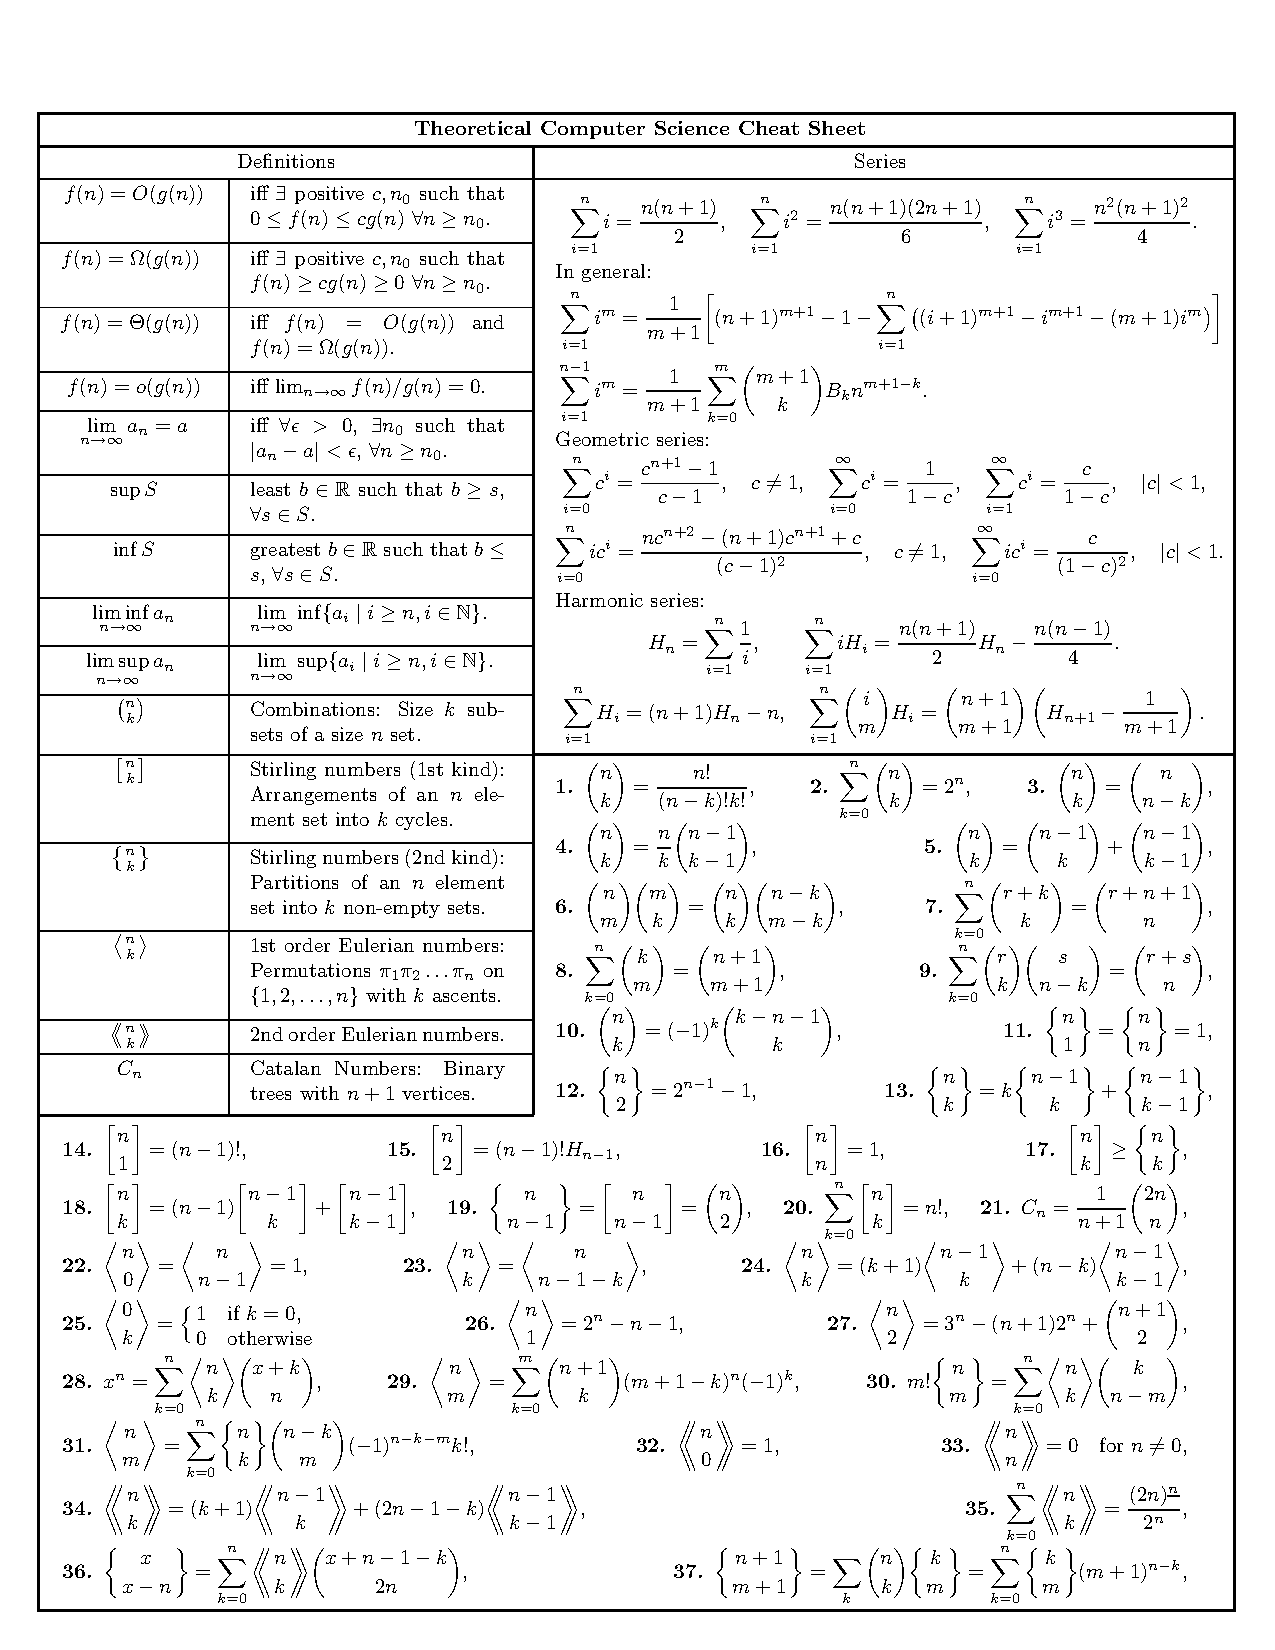
\includepdf[landscape=true,pages={1-5},pagecommand={\thispagestyle{fancy}}]{cheat}

\end{document}